\documentclass[tikz,convert=false]{standalone}
\begin{document}
  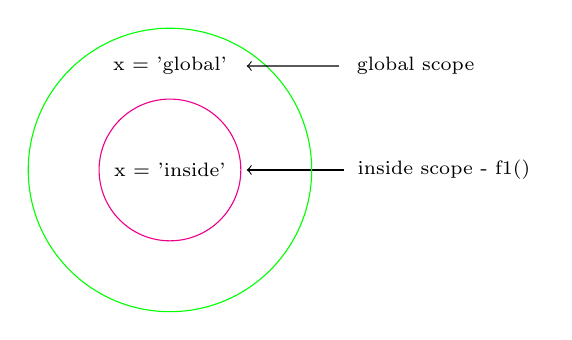
\begin{tikzpicture}[scale=0.6]
    % inside scope
    \draw [magenta] (0,0) circle [radius=1.5] node (i1) {};
    \node [draw=none,align=center, font=\scriptsize,text width = 2.3cm, name=i2] at (5.8,0) {inside scope - f1()};
    \node[draw=none,align=center, font=\scriptsize,text width = 1.7cm, name=i3] at (0,0) {x = 'inside'};
    \draw [->] (i2) -- (i3);

    % global scope
    \draw [green] (0,0) circle [radius=3]  node (g1) {};
    \node [draw=none,align=center, font=\scriptsize,text width = 1.7cm, name=g2] at (5.2,2.2) {global scope};
    \node [draw=none,align=center, font=\scriptsize,text width = 1.7cm, name=g3] at (0,2.2) {x = 'global'};
    \draw [->] (g2) -- (g3);
  \end{tikzpicture}
\end{document}